\documentclass{article}
\usepackage{amsfonts, amsmath}

\usepackage{geometry}
\geometry{a4paper, portrait, margin=1in}

\usepackage{enumitem}

\usepackage{tikz}

%% TODO: make it two columns??

\title{Exercises from \\
  Linear Algebra and Learning from Data\\
  by Gilbert Strang
}

\newcommand{\sep}{\begin{center}$\heartsuit$~$\diamondsuit$~$\clubsuit$~$\spadesuit$\end{center}}
\newcommand{\sol}{\begin{center}\small{Solution:}\end{center}}
\newcommand{\vect}[1]{\ensuremath{\boldsymbol{#1}}}

\newcounter{prblm}
\newcommand{\problemset}[1]{\setcounter{prblm}{0}\section*{#1}}
\newcommand{\problem}[1]{
  \begingroup
  \ifnum\value{prblm} > 0 \sep \fi
  \stepcounter{prblm}
  \noindent\textbf{\arabic{prblm}} #1
  \sol
  \endgroup
}

\begin{document}
\maketitle

\problemset{Problem Set I.1}

\problem{Give an example where a combination of three nonzero vectors in $\mathbb{R}^4$ is the zero vector. Then write your example in the form $Ax = 0$. What are the shapes of $A$ and $x$ and 0?}

\begin{displaymath}
2 \begin{bmatrix} 1 \\ 2 \\ 3 \\ 4 \end{bmatrix}
+ \begin{bmatrix} 4 \\ 5 \\ 6 \\ 7 \end{bmatrix}
- 3 \begin{bmatrix} 2 \\ 3 \\ 4 \\ 5 \end{bmatrix}
= \begin{bmatrix} 0 \\ 0 \\ 0 \\ 0 \end{bmatrix}
\end{displaymath}

\begin{displaymath}
\begin{bmatrix} 1 & 4 & 2 \\ 2 & 5 & 3 \\ 3 & 6 & 4 \\ 4 & 7 & 5 \end{bmatrix}
\begin{bmatrix} 2 \\ 1 \\ -3 \end{bmatrix}
= \begin{bmatrix} 0 \\ 0 \\ 0 \\ 0 \end{bmatrix}
\end{displaymath}

The shape of $A$ is 4x3, the shape of $x$ is 3x1, the shape of 0 is 4x1.

\begin{verbatim}
import numpy as np

a = [[1,4,2],[2,5,3],[3,6,4],[4,7,5]]
x = [2,1,-3]

b = np.dot(a,x)
assert(b == np.zeros(4))
print(b)
\end{verbatim}


\problem{Suppose a combination of the columns of A equals a different combination of those columns. Write that as Ax = Ay. Find two combinations of the columns of A that
equal the zero vector (in matrix language, find two solutions to Az = 0).}


\begin{displaymath}
-2 \begin{bmatrix} 1 \\ 2 \\ 3 \\ 4 \end{bmatrix}
- \begin{bmatrix} 4 \\ 5 \\ 6 \\ 7 \end{bmatrix}
+ 3 \begin{bmatrix} 2 \\ 3 \\ 4 \\ 5 \end{bmatrix}
= \begin{bmatrix} 0 \\ 0 \\ 0 \\ 0 \end{bmatrix}
\end{displaymath}

\begin{displaymath}
4 \begin{bmatrix} 1 \\ 2 \\ 3 \\ 4 \end{bmatrix}
+ 2 \begin{bmatrix} 4 \\ 5 \\ 6 \\ 7 \end{bmatrix}
- 6 \begin{bmatrix} 2 \\ 3 \\ 4 \\ 5 \end{bmatrix}
= \begin{bmatrix} 0 \\ 0 \\ 0 \\ 0 \end{bmatrix}
\end{displaymath}

\begin{verbatim}
import numpy as np

a = [[1,4,2],[2,5,3],[3,6,4],[4,7,5]]
z1 = [-2, -1, 3]
z2 = [4, 2, -6]

b1 = np.dot(a, z1)
b2 = np.dot(a, z2)
assert(b1 == np.zeros(4))
assert(b2 == np.zeros(4))
print(f"{b1=} {b2=}")
\end{verbatim}


\problem{(Practice with subscripts) The vectors $\vect{a}_1, \vect{a}_2, \ldots , \vect{a}_n$ are in $m$-dimensional space $\mathbb{R}^m$, and a combination $c_1\vect{a}_1 + \cdots + c_n\vect{a}_n$ is the zero vector. That statement is at the vector level. 
\begin{enumerate}[label=(\arabic*)]
\item Write that statement at the matrix level. Use the matrix $A$ with the $\vect{a}$'s in its columns and use the column vector $\vect{c} = (c_1, \ldots, c_n)$.
\item Write that statement at the scalar level. Use subscripts and sigma notation to add up numbers. The column vector $\vect{a}_j$ has components $\vect{a}_{1j}, \vect{a}_{2j}, \ldots, \vect{a}_{mj}$.
\end{enumerate}}


\begin{displaymath}
  \begin{bmatrix}
    a_{1,1} ~ \ldots ~ a_{1,n} \\
    a_{2,1} ~ \ldots ~ a_{2,n} \\
    \vdots ~ \ddots ~ \vdots \\
    a_{m,1} ~ \ldots ~ a_{m,n}
  \end{bmatrix}
  * \begin{bmatrix} c_1 \\ c_2 \\ \vdots \\ c_n \end{bmatrix}
  = \begin{bmatrix} 0 \\ 0 \\ \vdots \\ 0_m \end{bmatrix}
\end{displaymath}

\begin{displaymath}
  \sum_{j=1}^{n} a_{i,j} * c_j = 0 ~ \text{for i in 1\ldots m}
\end{displaymath}


\problem{Suppose $A$ is the 3 by 3 matrix $\mathbf{ones}(3, 3)$ of all ones. Find two independent vectors $\vect{x}$ and $\vect{y}$ that solve $A\vect{x} = 0$ and $A\vect{y} = 0$. Write that first equation $A\vect{x} = 0$ (with numbers) as a combination of the columns of $A$. Why don't I ask for a third independent vector with $A\vect{z} = 0$?}


\begin{displaymath}
  x = \begin{bmatrix} 1 \\ -1 \\ 0 \end{bmatrix}
  ~~~
  \begin{bmatrix} 1 ~ 1 ~ 1 \\ 1 ~ 1 ~ 1 \\ 1 ~ 1 ~ 1 \end{bmatrix} \begin{bmatrix} 1 \\ -1 \\ 0 \end{bmatrix} = \begin{bmatrix} 0 \\ 0 \\ 0 \end{bmatrix}
\end{displaymath}

\begin{displaymath}
  y = \begin{bmatrix} 1 \\ 1 \\ -2 \end{bmatrix}
  ~~~
  \begin{bmatrix} 1 ~ 1 ~ 1 \\ 1 ~ 1 ~ 1 \\ 1 ~ 1 ~ 1 \end{bmatrix} \begin{bmatrix} 1 \\ 1 \\ -2 \end{bmatrix} = \begin{bmatrix} 0 \\ 0 \\ 0 \end{bmatrix}
\end{displaymath}

Any other $\vect{z}$ vector that solves the equation $A\vect{z}=0$ is a linear combination of $\vect{x}$ and $\vect{y}$.

\begin{verbatim}
import numpy as np

ones = [[1,1,1],[1,1,1],[1,1,1]]
x = [1,-1,0]
y = [1,1,-2]

b1 = np.dot(ones, x)
b2 = np.dot(ones, y)
zeros = np.zeros(3, dtype='int')
assert((b1 == zeros).all())
assert((b2 == zeros).all())
print(f"{b1=} {b2=}")
\end{verbatim}


\problem{The linear combinations of $\vect{v} = (1, 1, 0)$ and $\vect{w} = (0, 1, 1)$ fill a plane in $\mathbb{R}^3$.
\begin{enumerate}[label=(\alph*)]
\item Find a vector $\vect{z}$ that is perpendicular to $\vect{v}$ and $\vect{w}$. Then $\vect{z}$ is perpendicular to every vector $c\vect{v} + d\vect{w}$ on the plane: $(c\vect{v} + d\vect{w})^T \vect{z} = c\vect{v}^T\vect{z} + d\vect{w}^T\vect{z} = 0 + 0$. 
\item Find a vector $\vect{u}$ that is not on the plane. Check that $\vect{u}^T\vect{z} \not= 0$.
\end{enumerate}}


\begin{displaymath}
  \vect{z} = \begin{bmatrix} 1 \\ -1 \\ 1 \end{bmatrix}
  ~~~
  \vect{u} = \vect{v} + \vect{z} = \begin{bmatrix} 1 \\ 1 \\ 0 \end{bmatrix} + \begin{bmatrix} 1 \\ -1 \\ 1 \end{bmatrix} = \begin{bmatrix} 2 \\ 0 \\ 1 \end{bmatrix}
\end{displaymath}
\begin{displaymath}
  \vect{u}^T\vect{z} = \begin{bmatrix} 2 ~ 0 ~ 1 \end{bmatrix} \begin{bmatrix} 1 \\ 0 \\ 1 \end{bmatrix} = 3
\end{displaymath}

\begin{verbatim}
import numpy as np

v = [1,1,0]
w = [0,1,1]
z = [1,-1,1]
u = np.add(v,z)
z_dot_u = np.dot(z,u)

def project(a, b):
   return np.dot(a, b) / np.linalg.norm(a)

assert(project(v,z) == 0.0)
assert(project(w,z) == 0.0)

assert(z_dot_u != 0)

m1 = [v,w,z]
m2 = [v,w,u]

rank1 = np.linalg.matrix_rank(m1)
rank2 = np.linalg.matrix_rank(m2)

assert(rank1 == 3)
assert(rank2 == 3)

print(f"{z=} {u=} {z_dot_u=}")
\end{verbatim}


\problem{If three corners of a parallelogram are (1, 1), (4, 2), and (1, 3), what are all three of the possible fourth corners? Draw two of them.}

The three possible fourth corners are:
\begin{gather*}
  (1,1) + ((4,2) - (1,3)) = (4,0) \\
  (4,2) + ((1,3) - (1,1)) = (4,4) \\
  (1,3) + ((1,1) - (4,2)) = (-2, 2) \\
\end{gather*}

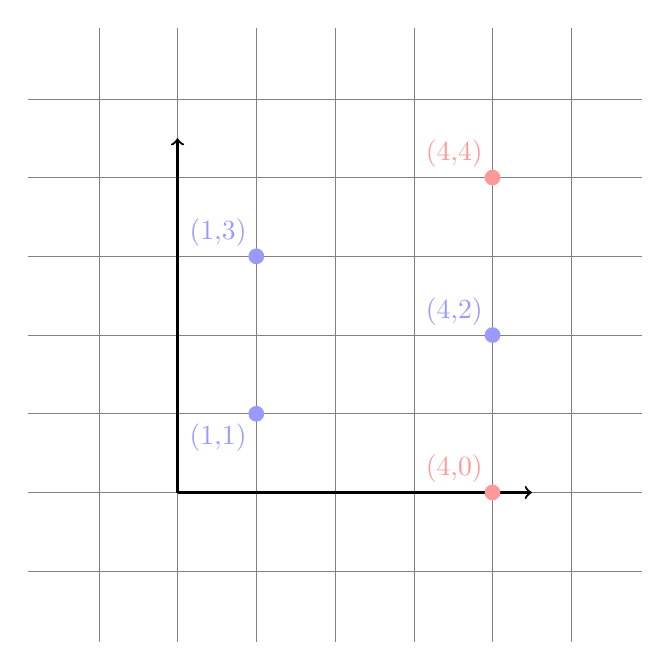
\begin{tikzpicture}
  \draw[step=1cm,gray,very thin] (-1.9,-1.9) grid (5.9,5.9);
  \draw[thick,->] (0,0) -- (4.5,0);
  \draw[thick,->] (0,0) -- (0,4.5);
  \fill[blue!40!white] (1,1) circle (1mm) node[anchor=north east] {(1,1)};
  \fill[blue!40!white] (4,2) circle (1mm) node[anchor=south east] {(4,2)};
  \fill[blue!40!white] (1,3) circle (1mm) node[anchor=south east] {(1,3)};
  \fill[red!40!white]  (4,0) circle (1mm) node[anchor=south east] {(4,0)};
  \fill[red!40!white]  (4,4) circle (1mm) node[anchor=south east] {(4,4)};
\end{tikzpicture}


\problem{Describe the column space of $A = [\vect{v} ~ \vect{w} ~ \vect{v} + 2\vect{w}]$. Describe the nullspace of $A$: all vectors $\vect{x} = (x1, x2, x3)$ that solve $A\vect{x} = 0$. Add the "dimensions" of that plane (the column space of $A$) and that line (the nullspace of $A$):
  \begin{center}{\textbf{dimension of column space + dimension of nullspace = number of columns}}\end{center}}

\end{document}
